%% SECTION HEADER /////////////////////////////////////////////////////////////////////////////////////
\section{Damage indices}
\label{sec:di}

%% SECTION CONTENT ////////////////////////////////////////////////////////////////////////////////////
In the dissertation, six damage indices are analysed based on the signal envelope in the time - domain registered by the sensor.
All of them are considered in three options: (i) the full-length of the signal, (ii) the first wave packet of the \ac{s0}, (iii) the first wave packet of the \ac{a0}.
The analysis will consider signals at 50, 100 and 150 \unit{\kHz}, with the last frequency excluded for the \ac{a0}, because, as indicated in section~\ref{sec:resuls}, this mode is masked by reflections of the \ac{s0}.
The wave packets are extracted by windowing the full-length signals with a flattened Gaussian window in the form:
\begin{eqnarray}
	g(t)= \mathrm{exp}\left(-\left(\frac{t-t_0}{w_g}\right) ^{n}\right),
	\label{eq:psi_g}
\end{eqnarray}
where \(t_0\) and \(w_g=0.5N_c/f_c\) are the center point and the half-width of the window, respectively, and  \(n\) determines the slope of the window.
The usage of the window is pictured in Fig.~\ref{fig:windows}.
\begin{figure}[!tbh]
	\begin{center}
		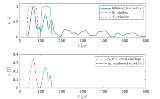
\includegraphics[width=0.95\textwidth]{Chapter_7/windows}
	\end{center}
	\caption{Windows}
	\label{fig:windows}
\end{figure}


The following time-domain indices presented in \cite{torkamani2014novel, moix2016damage} are take into consideration: \ac{p2p}, \ac{saps}, \ac{sapr}, \acf{rmsd}, \ac{eng} and \ac{cc}.

\begin{eqnarray}
	\mathrm{P2P} & = & \left(\mathrm{max}(e_H) - \mathrm{max}(e_D)\right)\\
	\mathrm{SAPS} & = & 1 - \left(\frac{\mathrm{max}(e_H)-\mathrm{max}(e_D)}{\mathrm{max}(e_H)}\right)^2,\\
	\mathrm{SAPR} & = & \frac{\mathrm{max}(e_H)}{\mathrm{max}(e_D)},\\
	\mathrm{RMSD} & = & 1 - \sqrt{\frac{\sum_{i=1}^{n}\left[e_D-e_H\right]^2}	{\sum_{i=1}^{n}e_H^2}},\\
	\mathrm{ENG} & = & 1 -  \frac{\sum_{i=1}^{n}{e_D^2}-\sum_{i=1}^{n}{e_H^2}}{\sum_{i=1}^{n}{e_H^2}},\\
	\mathrm{CC} & = & \frac{n\sum_{i=1}^{n}e_De_H-\sum_{i=1}^{n}e_D\sum_{i=1}^{n}e_H}{\sqrt{n\sum_{i=1}^{n}e_D^2-\left[\sum_{i=1}^{n}e_D\right]^2}\sqrt{n\sum_{i=1}^{n}e_H^2-\left[\sum_{i=1}^{n}e_H\right]^2}},
\end{eqnarray}
where \(e_H\) and \(e_D\) are the envelope of the signal registered by the sensor for the healthy and damaged state of the sample, respectively, and \(n\) is the length of the signal.
The \ac{p2p}, \ac{saps}, \ac{sapr}  are based on the difference between amplitudes of the monitored and the baseline state.
The \ac{rmsd} measures the error between baseline and damaged, \ac{eng} compares the difference of the sensor responses energy and \ac{cc} is the index based on Pearson correlation coefficient.

\begin{figure}[!tbh]
	\begin{center}
		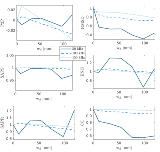
\includegraphics[width=0.95\textwidth]{Chapter_7/DI_full_full}
	\end{center}
	\caption{The \acfp{di} obtained with the \acf{fcgm} based on full-length signals.}
	\label{fig:DI_full_full}
\end{figure}
\begin{figure}[!tbh]
	\begin{center}
		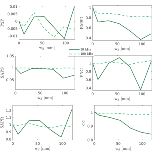
\includegraphics[width=0.95\textwidth]{Chapter_7/DI_full_A0}
	\end{center}
	\caption{The \acfp{di} obtained with the \acf{fcgm} based on \acs{a0} windowed signal.}
	\label{fig:DI_full_A0}
\end{figure}
\begin{figure}[!tbh]
	\begin{center}
		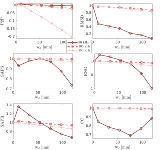
\includegraphics[width=0.95\textwidth]{Chapter_7/DI_full_S0}
	\end{center}
	\caption{The \acfp{di} obtained with the \acf{fcgm} based on \acs{s0} windowed signal.}
	\label{fig:DI_full_S0}
\end{figure}

The \acp{di} based on full-length signals derived from simulations with the \ac{fcgm} are presented in Fig.~\ref{fig:DI_full_full}.
The damage was modelled by removing the core cells.
Most \acp{di} for 50 \unit{\kHz} are undetermined.
The exception is \ac{cc} and \ac{rmsd} excluding the most significant damage. 
This is due to the fact that a low-frequency wave, according to work of Tian et al. \cite{tian2015wavenumber} up to 100 \unit{\kHz}, propagates through the entire thickness of the \ac{hsc}.
Consequently, the effect of damage on wave propagation is more complex than the high-frequency modes.
The high-frequency wave propagates mainly through the skin of the panel, so changes in the signal recorded by the sensor in the damaged sample are mainly caused by the wave leakage effect. 

The \acp{di} based on the windowed signals are shown in Fig.~\ref{fig:DI_full_A0} and Fig.~\ref{fig:DI_full_S0} for the \ac{a0} and \ac{s0} window, respectively.
It should be mentioned that \acp{di} for 150 \unit{\kHz} are omitted in Fig.~\ref{fig:DI_full_A0}, due to the masking of this mode by the \ac{s0} reflections.
The characteristics of the indices are consistent with the related indices determined for the full-length signals.
However, the values of most windowed signals are lower than those of whole signals.
In addition, the \ac{s0} window-based \acp{di} have lower values than the \ac{a0} windowed signals.
It is because dominant displacements of the \ac{s0} are in-plane of the skin, so a smaller portion of the energy of the wave leak into the core thru the healthy region.
In the case of the full-length response, the \ac{a0} is registered, which dominant displacements are out of the plate, making this mode more sensible for damage like disbonds or delamination.
Moreover, the smallest damage impact is noticeable for signals with a frequency of 150 \unit{\kHz}.

Accordingly, the following indicators are chosen for further consideration: \ac{cc} and \ac{rmsd}, both in the case of full-length and for frequency of 50 and 100 \unit{\kHz}.
Windowed signals are not accounted because changes are less than for full-length.
Those indices are compered with the \acp{di} obtained with the damage modelled by removing the interface elements and the results from simulations based on the \ac{hcgm} with both damage models.
The comparison is shown in Fig.~\ref{fig:DI_all}.
It can be seen that the damage model has an effect only for both indices with a frequency of 50 \unit{\kHz}, while the differences are negligible for 100 \unit{\kHz}.
However, significant differences are found for two core models, especially at 100 \unit{\kHz}.
\begin{figure}[!tbh]
	\begin{center}
		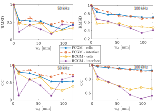
\includegraphics[width=0.95\textwidth]{Chapter_7/DI_all}
	\end{center}
	\caption{Comparison of the chosen \acfp{di} for the various models of the core and damage: solid line the \acf{fcgm} with removed core cells, dashed line the \acf{fcgm} with removed interface elements, dash-dot line the \acf{hcgm} with removed core cells, dotted line the \acf{hcgm} with removed interface elements.}
	\label{fig:DI_all}
\end{figure}
